% CSC311 Summer 2026 Final Project - Option 2
% Compile: pdflatex final_report.tex  (run twice)
\documentclass[10pt]{article}

\usepackage[letterpaper,margin=0.78in]{geometry}
\usepackage{graphicx}
\usepackage{booktabs}
\usepackage{amsmath}
\usepackage{amssymb}
\usepackage{url}
\usepackage[hidelinks]{hyperref}
\usepackage{caption}
\usepackage{tikz}
\usetikzlibrary{arrows.meta, positioning}

\captionsetup{font=small}
\setlength{\parskip}{1pt}
\linespread{0.97}
% tighter spacing around floats, to fit the page budget
\setlength{\textfloatsep}{9pt plus 2pt minus 2pt}
\setlength{\floatsep}{9pt plus 2pt minus 2pt}
\setlength{\intextsep}{9pt plus 2pt minus 2pt}
\setlength{\abovecaptionskip}{4pt}
% let more floats sit on a page: the defaults are too strict for this many
\setcounter{topnumber}{3}
\setcounter{bottomnumber}{2}
\setcounter{totalnumber}{4}
\renewcommand{\topfraction}{0.92}
\renewcommand{\bottomfraction}{0.7}
\renewcommand{\textfraction}{0.06}
\renewcommand{\floatpagefraction}{0.75}

\title{\vspace{-1.6em}\textbf{Can Machine Learning Help a Stock-Trading Strategy?}\\
\large Testing 8 versions of ``pairs trading'' on 10 years of real market data}

\author{[Name 1] \quad [Name 2] \quad [Name 3] \\
\normalsize CSC311 Summer 2026 Final Project (Option 2)\\
\normalsize Code: \url{https://github.com/eram-111/pair_trading}}
\date{}

\begin{document}
\maketitle

\begin{abstract}
\noindent
Some stocks normally move together. When two drift apart, a classic strategy bets
the gap will close. The hard part is knowing \emph{which} gaps are worth betting
on --- a machine-learning problem: predict whether a gap will close, then trade
only when confident. We built 8 versions --- 2 ways of choosing pairs $\times$ 4
ways of deciding to trade --- and tested all of them identically on 10 years of
real prices. The models learn something real: on data they had never seen they
rank opportunities better than guessing. But none makes money after fees, because
the edge is worth about 39 cents per \$100 traded and the fees cost 40. Two
findings surprised us more than the returns did: a good accuracy score makes our
models look useful when they are not, and the version that looked best during
development was among the worst on the final test.
\end{abstract}

\section{Introduction}

Chevron and Exxon are both oil companies. When oil prices move, both stocks
usually move the same way. So if Chevron jumps 3\% one week and Exxon does not
move at all, something unusual has happened. Either there is real news about one
company, or the gap is just noise and the two will drift back together.

\emph{Pairs trading} is a strategy that bets on the second story. When the gap
opens, you buy the one that fell behind and bet against the one that ran ahead.
If they come back together, you win on both sides. If they do not, you lose. It
is one of the oldest computer-driven trading strategies and it used to work well
\cite{gatev2006}.

The problem is that most gaps do \textbf{not} close --- in our data only about 1
in 4 does. So the interesting question is \textbf{``when a gap opens, is this one
worth trading?''} That is a prediction problem, which is what machine learning is
for. This report asks whether adding machine learning actually helps. To answer
fairly we built 8 versions differing in only two ways, ran all 8 through identical
code, looked at the test data exactly once, and put everything online.

\begin{table}[!ht]
\small
\caption{The names we use. The 8 versions we test are every combination of a
\textbf{track} (how pairs are chosen) with a \textbf{model} (how we decide to
trade), so ``Track~A / E3'' means pairs picked by price movement, traded when a
neural network says so.}
\label{tab:names}
\begin{tabular}{@{}p{0.17\textwidth}p{0.76\textwidth}@{}}
\toprule
\multicolumn{2}{@{}l}{\textbf{The two ways of choosing pairs}} \\
\midrule
Track A & Stocks that \emph{move} alike, after removing the market-wide swings
that push everything at once. \\
Track B & Stocks whose \emph{businesses} look alike: similar profits, growth and
valuation. Price history is not used. \\
\midrule
\multicolumn{2}{@{}l}{\textbf{The four ways of deciding to trade}} \\
\midrule
E0 & Trades every gap. No learning at all --- our baseline. \\
E1 & Logistic regression: draws one straight dividing line between gaps that
close and gaps that do not. \\
E2 & Gaussian discriminant analysis: learns what each outcome typically looks
like, then works backwards with Bayes' rule. \\
E3 & A small neural network: the only one that can learn curved patterns. \\
\midrule
\multicolumn{2}{@{}l}{\textbf{Words}} \\
\midrule
Spread, $z$-score & How far apart the two stocks have drifted, and how unusual
that is. $z=2$ means ``much bigger than normal''. \\
Trigger & A moment when a gap gets big enough to consider trading. \\
Basis point & One hundredth of 1\%. 40 bps = 40 cents per \$100 traded. \\
Accuracy & How often a yes/no call is right. \\
Precision & Of the gaps a model chose to trade, the share that actually closed. \\
Win rate & Share of trades that ended up making money. \\
AUC & Chance the model scored a gap that closed above one that did not.
$0.5$ = random guessing, $1.0$ = perfect. \\
Breakeven & The fee level at which a version stops making money. Above 10
means it survives the fees we assume. \\
\bottomrule
\end{tabular}
\end{table}

\section{What other people have done}

Gatev and co-authors \cite{gatev2006} wrote the paper that made this strategy
famous: pick pairs whose prices had historically tracked each other, trade when
they drift apart, and close when they re-converge. It made real money on
1962--2002 US stocks. Later researchers found those profits shrinking as the
strategy became crowded and fees ate the rest.

Two papers improved how pairs are chosen, and they are the two tracks we compare.
Avellaneda and Lee \cite{avellaneda2010} first strip out the market-wide
movements that push every stock at once, and look only at what is left for each
stock (our Track~A). Zhang and co-authors \cite{zhang2014} instead group
companies by what the \emph{business} looks like --- profitability, growth,
valuation --- rather than by price history (our Track~B); we also borrow their
rules for turning groups into pairs. More recent work adds machine learning:
clustering for choosing pairs \cite{sarmento2020, rotondi2024} and classifiers
for choosing when to enter \cite{ekinci2025}. We are not proposing a new method.
We are trying to measure honestly whether the machine-learning part helps, by
holding everything else fixed and adding a control experiment (Section~6.3) that
this literature largely omits.

For splitting data we follow López de Prado \cite{lopezdeprado2018}. In ordinary
machine learning you can shuffle your examples; with trading data you cannot,
because an example from Monday already ``knows'' Tuesday's prices. We split by
date and discard examples near the boundaries.

\section{How our system works}

\subsection{The pipeline}

Figure~\ref{fig:pipeline} shows the whole system: prices go in at the left and
trading results come out at the end. The grey boxes are shared by all 8 versions
--- same code, same settings, same random seed --- and only the white boxes
change. So if one version beats another, it is because of the thing we changed,
not because one got a better backtest.

\begin{figure}[!ht]
\centering
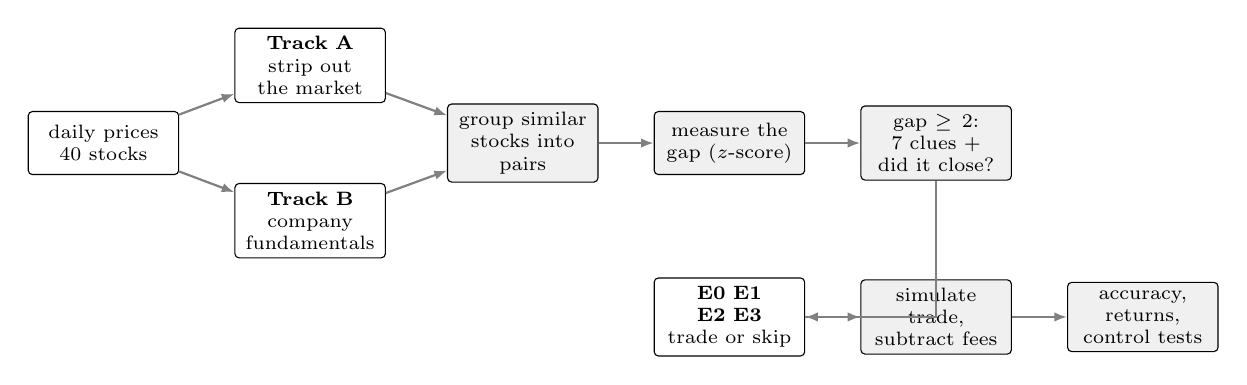
\begin{tikzpicture}[
  box/.style={draw, rounded corners=1.5pt, align=center, font=\scriptsize,
              minimum height=8mm, inner sep=3pt, text width=17mm},
  shared/.style={box, fill=black!6},
  arrow/.style={-{Latex[length=1.6mm]}, gray, thick}
]
% row 1: prices, the two tracks, pairs
\node[box] (prices) {daily prices\\ 40 stocks};
\node[box, above right=1mm and 7mm of prices] (pca) {\textbf{Track A}\\ strip out\\ the market};
\node[box, below right=1mm and 7mm of prices] (chars) {\textbf{Track B}\\ company\\ fundamentals};
\node[shared, right=7mm of prices, xshift=27mm] (cluster) {group similar\\ stocks into\\ pairs};
\node[shared, right=7mm of cluster] (spread) {measure the\\ gap ($z$-score)};
\node[shared, right=7mm of spread] (trig) {gap $\ge 2$:\\ 7 clues +\\ did it close?};

% row 2: models, engine, results
\node[box, below=13mm of spread] (models) {\textbf{E0 E1 E2 E3}\\ trade or skip};
\node[shared, right=7mm of models] (engine) {simulate trade,\\ subtract fees};
\node[shared, right=7mm of engine] (metrics) {accuracy,\\ returns,\\ control tests};

\draw[arrow] (prices) -- (pca);
\draw[arrow] (prices) -- (chars);
\draw[arrow] (pca) -- (cluster);
\draw[arrow] (chars) -- (cluster);
\draw[arrow] (cluster) -- (spread);
\draw[arrow] (spread) -- (trig);
\draw[arrow] (trig.south) |- (models.east);
\draw[arrow] (models) -- (engine);
\draw[arrow] (engine) -- (metrics);
\end{tikzpicture}
\caption{Our system, left to right then down. Grey boxes are identical for all 8
versions; only the white boxes --- how pairs are chosen, and which model decides
--- change. That is what makes the comparison fair.}
\label{fig:pipeline}
\end{figure}

\subsection{One trade, start to finish}

Figure~\ref{fig:method} shows a real trade from our test data. Two energy stocks
drift apart (top). We measure that gap as a $z$-score (bottom): when it crosses
2, the gap is unusually large and we call that a \textbf{trigger}. We wait one
day (so we could only ever trade on information we already had), then bet on the
gap closing. We close the trade when the gap shrinks, or after 5 days if nothing
happens.

Every trigger becomes one training example. The \textbf{answer} to predict is:
did the gap shrink by half within 5 days? (Yes about 24\% of the time.) The
\textbf{clues} are 7 numbers: how big the gap is, how jumpy the pair usually is,
whether the gap is still widening, how volatile the market is, trading volume,
days since this pair last triggered, and how stable the pairing is.

\begin{figure}[!ht]
\centering
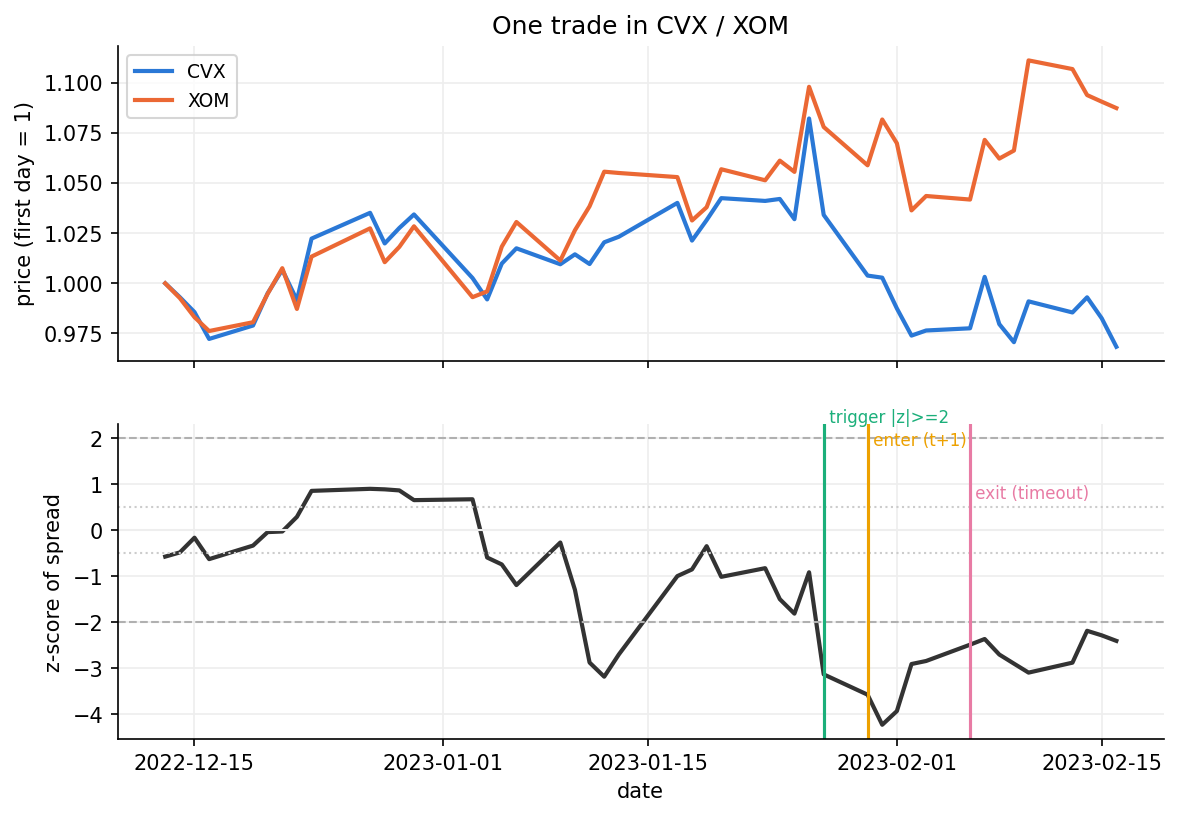
\includegraphics[width=0.48\textwidth]{../results/figures/method_example.png}
\caption{A real trade. Top: two stocks drift apart. Bottom: the gap crosses our
threshold, we enter the next day, and exit when it closes.}
\label{fig:method}
\end{figure}

\subsection{Data and how we tested}

We used 40 large US companies (10 each from technology, banking, energy and
consumer goods), daily prices 2015--2024; Track~B additionally uses 19 business
measurements per company per quarter.



We split by time: \textbf{2015--2020} to learn from (1{,}074 opportunities on
Track~A, 1{,}122 on Track~B), \textbf{2021--2022} to choose settings (345 / 378),
and \textbf{2023--2024} to test (356 / 324); about 1\% of examples sitting on the
boundaries are discarded, because a trade starting just before a cut-off would
have its outcome decided on the other side. Roughly a quarter of gaps close in
every period --- the number any model must beat. We looked at the test years
exactly once, at the very end, after everything was locked; if you keep checking
your test data and adjusting, you end up fooling yourself and the score stops
meaning anything.

Trading is not free. Every trade pays a fee on both stocks, going in and coming
out. We assume 10 basis points per leg, which totals \textbf{40 basis points
(0.40\%) per round trip}. We report results both with and without this fee,
because the difference between them turned out to be the whole story.

\begin{table}[!ht]
\centering
\small
\caption{\textbf{Did the models predict well?} Test years only. Each model's
precision should be compared with its own track's ``trade all'' row, which is the
rate for gaps in general. Bracket = 95\% range. Read with Section~6.2.}
\label{tab:predict}
\begin{tabular}{llrrrrl}
\toprule
Track & Model & Gaps offered & Chose to trade & Accuracy & Precision & AUC [95\% range] \\
\midrule
A & E0 (trade all) & 356 & 356 (100\%) & 21\% & 21\% & --- \\
A & E1 (logistic) & 356 & 66 (19\%) & 71\% & 29\% & 0.546 \ [0.472, 0.625] \\
A & E2 (GDA) & 356 & 54 (15\%) & 73\% & \textbf{31\%} & 0.549 \ [0.474, 0.627] \\
A & E3 (neural net) & 356 & 60 (17\%) & 71\% & 25\% & 0.543 \ [0.470, 0.618] \\
\midrule
B & E0 (trade all) & 324 & 324 (100\%) & 24\% & 24\% & --- \\
B & E1 (logistic) & 324 & 106 (33\%) & 63\% & 29\% & 0.558 \ [0.487, 0.632] \\
B & E2 (GDA) & 324 & 103 (32\%) & 62\% & 28\% & 0.559 \ [0.488, 0.631] \\
B & E3 (neural net) & 324 & 84 (26\%) & 68\% & \textbf{35\%} & \textbf{0.577 \ [0.505, 0.649]} \\
\midrule
\multicolumn{2}{l}{\emph{Never trade at all}} & --- & 0 (0\%) & \textbf{79\%} & --- & --- \\
\bottomrule
\end{tabular}
\end{table}

\begin{table}[!ht]
\centering
\small
\caption{\textbf{Did the models make money?} Test years, average per trade in
basis points (100 bps = 1\%). ``After fees'' subtracts the 40 bps round trip.
Bracket = 95\% range. ``Beat luck'' compares each model with 1{,}000 random
strategies that trade equally often; 50 means indistinguishable from random.}
\label{tab:money}
\begin{tabular}{llrrlrr}
\toprule
Track & Model & Win rate & Before fees & After fees [95\% range] & Breakeven & Beat luck \\
\midrule
A & E0 (trade all) & 46\% & $+8.4$ & $-31.6$ \ $[-71, +7]$ & $+2.1$ & --- \\
A & E1 (logistic) & 52\% & $\mathbf{+38.7}$ & $\mathbf{-1.3}$ \ $[-111, +95]$ & $\mathbf{+9.7}$ & 76 \\
A & E2 (GDA) & 52\% & $+23.0$ & $-17.0$ \ $[-143, +102]$ & $+5.8$ & 61 \\
A & E3 (neural net) & 40\% & $-44.7$ & $-84.7$ \ $[-214, +35]$ & $-11.2$ & 11 \\
\midrule
B & E0 (trade all) & 39\% & $-31.6$ & $-71.6$ \ $[-116, -28]$ & $-7.9$ & --- \\
B & E1 (logistic) & 35\% & $-54.9$ & $-94.9$ \ $[-196, +8]$ & $-13.7$ & 19 \\
B & E2 (GDA) & 34\% & $-62.3$ & $-102.3$ \ $[-199, -0.2]$ & $-15.6$ & 15 \\
B & E3 (neural net) & 42\% & $+23.7$ & $-16.3$ \ $[-119, +85]$ & $+5.9$ & \textbf{90} \\
\midrule
\multicolumn{2}{l}{\emph{Never trade at all}} & --- & $0$ & $0$ & --- & --- \\
\bottomrule
\end{tabular}
\end{table}

\section{Two ways to pick pairs}

\textbf{Track A: pairs that move alike.} Following Avellaneda and Lee
\cite{avellaneda2010}, each day we take the last year of returns and use PCA to
find the few patterns explaining most of how all 40 stocks move together --- the
market and a few sector-like effects --- and subtract them out. What remains for
each stock is its own private movement, and that is what we track:
\begin{equation}
\varepsilon_{i,t} = r_{i,t} - \Big(\alpha_i + \textstyle\sum_{k=1}^{m}\beta_{ik} f_{k,t}\Big)
\end{equation}
Every month we group stocks by their factor loadings $\beta_i$ using $k$-means,
choosing the number of groups by silhouette score. This gives 120 regroupings and
201 pairs. \emph{Comparing the models here:} Track~A produced the best single
cell in the study (E1, essentially breakeven) and the worst (E3), so on the same
pairs the choice of model swung the result by more than 80 bps per trade.

\textbf{Track B: pairs that look alike.} Following Zhang and co-authors
\cite{zhang2014}, each quarter we take 19 measurements per company, clean them
(drop sparse columns, fill gaps with the median, standardise within the quarter),
compress them with PCA, and group companies that resemble each other as
\emph{businesses}. Price history plays no part. This gives 39 regroupings and 242
pairs. Both tracks then trade the same underlying gaps, so only the grouping
differs. \emph{Comparing the models here:} Track~B gave the best predictions in
the study (E3, the only AUC whose range excludes chance) and the only model to
clearly beat its random-strategy control --- but its two linear models were the
worst money-losers overall.

\section{Four ways to decide when to trade}

Table~\ref{tab:names} says what each model is; here is how each one works and how
it fared on the two tracks. All four see the same 7 clues and output a number
between 0 and 1 --- how likely this gap is to close --- and trade when that
number clears a cutoff $\tau$ we fixed by a rule set in advance.

\textbf{E0} learns nothing, so it is the bar the others must clear. It lost
$-31.6$ bps per trade on Track~A and $-71.6$ on Track~B: simply trading every gap
was worse than doing nothing on both tracks.

\textbf{E1} fits $\hat p = \sigma(w^\top x + b)$ with an L2 penalty and class
weights that correct for the 24\% base rate, choosing the penalty strength by
validation AUC. It is the natural first model here: with 7 clues and about 1{,}100
training examples, anything more flexible risks memorising. \emph{Across tracks}
it gave the best cell in the study on Track~A and one of the two worst on
Track~B --- the same model, opposite verdicts.

\textbf{E2} asks the question backwards. Rather than learning a boundary, it
assumes gaps that close and gaps that do not each form a bell-shaped cloud,
learns both clouds, and applies Bayes' rule. Assuming the clouds share a shape
makes its answer a straight line again --- so it should behave like E1, and it
does (Section~6.4). \emph{Across tracks} it tracks E1 almost exactly on both.

\textbf{E3} is a small network: 7 inputs, one hidden layer of 8 or 16 units, one
output, trained with early stopping. It is the only model that can bend its
boundary. \emph{Across tracks} it inverts E1's pattern --- worst on Track~A, best
on Track~B, where it produced the study's only convincing evidence of skill. That
flip, from the same model on the same 7 clues, is the clearest sign that with this
little data the choice of model and the choice of pairs interact in ways we cannot
separate.

\section{Results}

\subsection{Nobody made money}

The two results tables ask different questions --- Table~\ref{tab:predict}
whether a model \emph{knew} anything, Table~\ref{tab:money} whether that
knowledge was \emph{worth} anything --- and they get different answers, which is
the heart of this report.

Start with the money. After fees, all 8 versions lost. The best, Track~A with
logistic regression, lost $1.3$ bps per trade --- close enough to zero that we
cannot tell it apart from breaking even. Every 95\% range in that column contains
zero except Track~B's E0 and E2, so for six of the eight we cannot even be
confident they lost.

The ``before fees'' column shows why. The best edge anyone found was $+38.7$ bps per
trade. The fee is $40$ bps. That is the entire story of this project in two
numbers: \textbf{the strategy earns about 39 cents per \$100 traded, and costs 40
cents to trade}. Three of the 8 versions had a positive edge before fees; none
kept it afterwards.

Fees hit every version at exactly the same rate, so the only thing separating a
good strategy from a bad one is the size of the edge it starts with. The
breakeven column of Table~\ref{tab:money} says this directly: Track~A's E1
survives fees up to 9.7 bps and Track~B's E3 up to 5.9, both just short of the 10
we assume, and the other six never break even at any fee.

\subsection{Accuracy is a trap here (and this surprised us)}

The accuracy column of Table~\ref{tab:predict} looks like great news. Trading every gap is ``correct'' only
21\% of the time, and our models are correct 62--73\%. That looks like a huge
improvement.

It is not. The last row of Table~\ref{tab:predict} shows a strategy that
\textbf{never trades at all} is correct 79\% of the time --- better than every
model we built --- while earning nothing. Most gaps do not close, so ``skip'' is
usually right, and any cautious model racks up a high score by skipping. Accuracy
rewards caution, not usefulness.

This is why we report AUC and actual returns as well. AUC ignores how often each
answer occurs and only asks whether the model \emph{ranks} good opportunities
above bad ones. On that measure all six learned cells score 0.543--0.577, which is
genuinely better than the 0.5 of random guessing, and for Track~B's neural network
the confidence interval $[0.505, 0.649]$ stays above 0.5. So the models did learn
something --- accuracy just was not the right way to see it.

\subsection{Trading less is not the same as choosing better}

Every model trades far less than E0 (60--106 trades instead of 324--356). Since
every trade costs money, trading less automatically improves results, even with
no skill whatsoever. So how much of the improvement is skill?

To find out we built 1{,}000 fake strategies per model. Each trades exactly as
often as the real one, in the same months, but picks \emph{at random} which gaps
to take. Figure~\ref{fig:controls} shows where the real model lands in that
crowd; the middle means its choices were no better than random.

Track~B's neural network lands at the 90th percentile --- better than 900 of
1{,}000 random imitators, the only strong evidence of real skill we found.
Track~A's logistic regression lands at 76. But Track~A's neural network lands at
11 and Track~B's linear models at 19 and 15, meaning they chose \emph{worse} than
picking at random. Without this test we would have reported E1's near-breakeven as
proof that learning works. With it, we can only say most of the gain came from
trading less.

\begin{figure}[!ht]
\centering
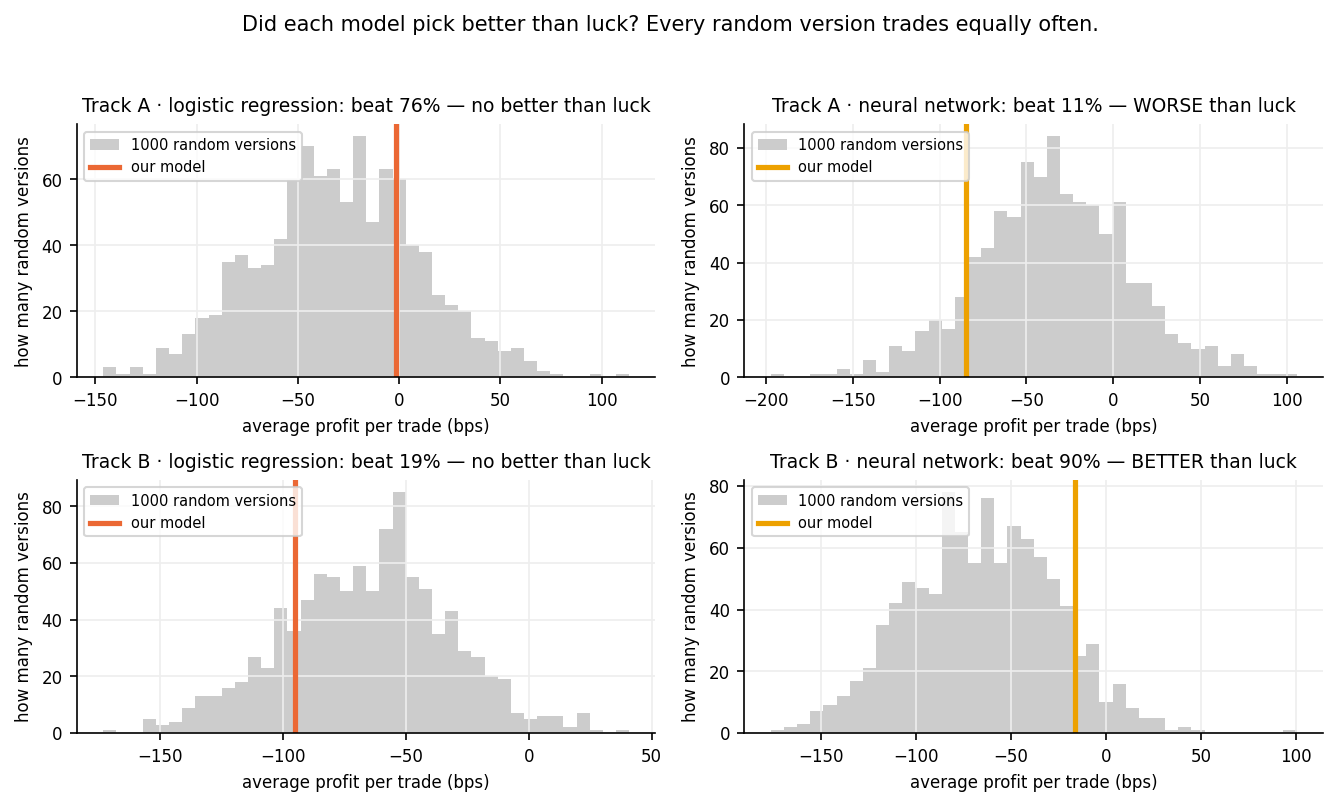
\includegraphics[width=0.60\textwidth]{../results/figures/controls_test.png}
\caption{Each model (coloured line) against 1{,}000 random strategies that trade
equally often (grey). Middle of the pile means the model's choices were no better
than random.}
\label{fig:controls}
\end{figure}

\subsection{The two linear models are the same model}

E1 and E2 come from different traditions --- one learns the boundary directly,
the other learns what each group looks like and works backwards --- yet they agree
almost everywhere: test AUC 0.546 vs 0.549 on Track~A, 0.558 vs 0.559 on Track~B,
and development control ranks of 16 vs 17 and 89 vs 88.

This is not a coincidence, and it is one of our favourite results because the
course predicts it. When E2 assumes both groups have the same shape, its answer
simplifies into exactly the same form as E1's: a straight line. So the two methods
are two different ways of drawing the same kind of boundary, and on this data they
land in nearly the same place. Only E3, which can bend, behaves differently.

\subsection{What looked best in development was not best in the end}

Table~\ref{tab:flip} puts development results next to test results, and this
comparison taught us more than anything else in the project.

During development, Track~B looked like a clear winner: its logistic regression
earned $+29.9$ bps per trade and its neural network $+24.3$, both profitable after
fees, and both ranked 88--89 against their random controls. We were, briefly, very
pleased.

On the test years, those same frozen models earned $-94.9$ and $-16.3$ bps, and
the logistic regression's control rank collapsed from 89 to 19. Meanwhile Track~A's
logistic regression went the other way, from rank 16 up to 76.

Nothing was broken: the models were locked before we read the test data and the
code reproduces exactly. A few hundred trades is simply not enough to tell these
strategies apart --- the differences we were admiring were noise. We report it
prominently because it would have been easy to stop at development and write a
more exciting, wrong report.

\begin{table}[!ht]
\centering
\small
\caption{The same frozen models, before and after. ``Return'' is per trade in bps
after fees; ``Ctrl'' is the percentile against turnover-matched random
strategies. Track~B looked profitable in development and lost on test; Track~A's
E1 went the other way.}
\label{tab:flip}
\begin{tabular}{llrrrr}
\toprule
& & \multicolumn{2}{c}{Return (bps)} & \multicolumn{2}{c}{Ctrl (\%ile)} \\
\cmidrule(lr){3-4}\cmidrule(lr){5-6}
Track & Model & Dev & Test & Dev & Test \\
\midrule
A & E1 & $-62.5$ & $-1.3$ & 16 & 76 \\
A & E3 & $-23.8$ & $-84.7$ & 72 & 11 \\
B & E1 & $\mathbf{+29.9}$ & $\mathbf{-94.9}$ & 89 & 19 \\
B & E3 & $+24.3$ & $-16.3$ & 75 & 90 \\
\bottomrule
\end{tabular}
\end{table}

\section{What we take away}

Before concluding we checked the machinery itself: run on fake, randomly
generated prices where profit is impossible, the whole system lost money ($-51$
bps per trade) and no model beat a simple baseline --- so it is not secretly
peeking at the future. Four things stand out.

\textbf{1. The fees are the whole problem.} Every model found a real but tiny
edge, worth about 39 cents per \$100 traded, against a 40-cent cost. No amount of
extra machine learning closes a gap that size; you would need cheaper trading.

\textbf{2. A good accuracy score can mean nothing.} Our models are ``right'' 70\%
of the time and lose money, while doing nothing is right 79\% of the time.

\textbf{3. Doing less looks like skill.} Filtering improves results automatically
because trades cost money --- only the random-strategy comparison showed that
most of our models had no real selecting ability.

\textbf{4. Small tests lie.} The version that looked best in development was
among the worst on test; with a few hundred examples the gaps between strategies
are smaller than the noise.

\section{What is wrong with our study}

Our biggest weakness is size: 40 stocks over 10 years leaves only about 350 test
opportunities per track, which is the direct cause of the reversal in
Section~6.5. A much larger universe would be the single most valuable extension.
Our fee model is a flat charge, but real fees rise exactly when markets are
volatile --- which is when our triggers fire --- so our results are, if anything,
optimistic. We fixed the entry and exit rules by hand rather than learning them,
which other work treats as its own machine-learning problem \cite{ekinci2025}.
And our confidence ranges assume trades are independent when they overlap in time
and repeat the same pairs, so the true ranges are wider than we report.

\section{Conclusion}

We built 8 versions of a pairs-trading strategy differing in only two ways, ran
them through identical code, and looked at the test data once. The machine
learning worked a little --- every learned model ranked opportunities better than
chance on data it had never seen, one convincingly --- but none made money,
because the edge is about 39 basis points and trading costs 40. The lessons we
valued most were not about trading: a model can be ``70\% accurate'' and still be
worse than doing nothing, a strategy can look skilful when it is only being lazy,
and a result that looks strong on a few hundred examples can reverse on the next
few hundred. All our code is public.

\bigskip
\noindent\textbf{Contributions.} [Name 1]: literature review, report writing,
results analysis. [Name 2]: data pipeline, features, Track~B fundamentals, E1.
[Name 3]: pair-forming pipeline, trade simulator, evaluation code (metrics,
controls, fake-data test), E2 and E3.

\smallskip
\noindent\textbf{Note on E2.} E2 first used the true 24\% closing rate as its
starting assumption, which pushed every probability below our cutoff so it never
traded --- a mismatch with how E1 and E3 handle the same imbalance, not a flaw in
the method. We caught this during development, fixed it so all four models are
treated alike, and re-ran E2 afterwards.

\smallskip
\noindent\textbf{Course evaluations.} All team members have completed the course
evaluation. % TODO: confirm before submitting

\begin{thebibliography}{9}
\small
\bibitem{gatev2006}
Gatev, E., Goetzmann, W.~N., \& Rouwenhorst, K.~G. (2006).
Pairs Trading: Performance of a Relative-Value Arbitrage Rule.
\emph{The Review of Financial Studies}, 19(3), 797--827.

\bibitem{avellaneda2010}
Avellaneda, M., \& Lee, J.-H. (2010).
Statistical arbitrage in the US equities market.
\emph{Quantitative Finance}, 10(7), 761--782.

\bibitem{zhang2014}
Zhang, W., Dai, Z., Pan, B., \& Djabirov, M. (2014).
A Multi-factor Adaptive Statistical Arbitrage Model. arXiv:1405.2384.

\bibitem{lopezdeprado2018}
López de Prado, M. (2018).
\emph{Advances in Financial Machine Learning}. Wiley. (Ch.~7.)

\bibitem{sarmento2020}
Sarmento, S.~M., \& Horta, N. (2020).
Enhancing a Pairs Trading strategy with the application of Machine Learning.
\emph{Expert Systems with Applications}, 158, 113490.

\bibitem{rotondi2024}
Rotondi, F., \& Russo, F. (2024).
Machine Learning for Pairs Trading: a Clustering-based Approach.
SSRN Working Paper 5080998.

\bibitem{ekinci2025}
Ekinci, C., et al. (2025).
Machine learning for optimal threshold selection in high-frequency pairs trading.
\emph{Computational Economics}.
\end{thebibliography}

\end{document}
